\documentclass[11pt]{article}

\usepackage{../handout}
%\usepackage{upquote}
\usepackage[pdftex]{graphicx, color}

\input{../mymargins}

\begin{document}
\handout{7}{5}{Solutions to Written Assignment 2}

\begin{enumerate}

\item
Give a context-free grammar (CFG) for each of the following languages
over the alphabet $\Sigma = \{0, 1\}$:
\begin{enumerate}
\item All nonempty strings that start and end with the same symbol.
\begin{eqnarray*}
S & \rightarrow & 0 \mid 1 \mid 0A0 \mid 1A1 \\
A & \rightarrow & A0 \mid A1 \mid \varepsilon
\end{eqnarray*}
\item All strings that contain more $1$s than $0$s.
\begin{eqnarray*}
S & \rightarrow & A1 \mid MS \mid SMA \\
A & \rightarrow & A1 \mid \varepsilon \\
M & \rightarrow & \varepsilon \mid MM \mid 0M1 \mid 1M0
\end{eqnarray*}
\item All palindromes (a palindrome is a string that reads the same
forwards and backwards).
\begin{eqnarray*}
S & \rightarrow & \varepsilon \mid 0 \mid 1 \mid 0S0 \mid 1S1
\end{eqnarray*}
\end{enumerate}

\item Consider the following CFG.
\begin{eqnarray*}
S & \rightarrow & AED \mid F \\
A & \rightarrow & Aa \mid a \\
B & \rightarrow & Bb \mid b \\
C & \rightarrow & Cc \mid c \\
D & \rightarrow & Dd \mid d \\
E & \rightarrow & bEc \mid bc \\
F & \rightarrow & aFd \mid BC
\end{eqnarray*}

\begin{enumerate}

\item What is the language generated by this grammar?
\[
\{a^{i}b^{j}c^{k}d^{i} \mid (i \geq 0) \land (j, k > 0)\}
\cup \{a^{i}b^{j}c^{j}d^{k} \mid i, j, k > 0\}
\]

\item Show that this grammar is ambiguous by giving a string that can
be parsed in two different ways.  Draw both parse trees.

The string $abcd$ has the two parse trees shown in Figure \ref{ambig}.
\begin{figure}[htb]
\begin{center}
\input{ambig.latex}
\caption{Two parse trees for the string $abcd$.}
\label{ambig}
\end{center}
\end{figure}

\item Give an unambiguous grammar that generates the same language as
the grammar above.
\begin{eqnarray*}
S & \rightarrow & AM \mid MD \mid F \\
A & \rightarrow & Aa \mid a \\
B & \rightarrow & Bb \mid b \\
C & \rightarrow & Cc \mid c \\
D & \rightarrow & Dd \mid d \\
E & \rightarrow & bEc \mid bc \\
F & \rightarrow & aFd \mid BC \\
M & \rightarrow & aMd \mid aEd
\end{eqnarray*}

\end{enumerate}

\item The Cool Reference Manual, in Chapter 11, has the context-free
grammar defining the syntax for Cool.  Create the parse tree from the
grammar definition for the following class definition.

\begin{verbatim}
class FOO inherits BAR {
  i : Int <- 42;
  baz (x:Int) : Foo { i <- x + i }; 
};
\end{verbatim}

Figure \ref{classparse} shows a sample parse tree for this class
definition.  In the Cool Reference Manual, the specification of the
syntax for Cool is not given as a pure CFG, and so some productions
have been introduced here to capture the regular expression notation
used in the specification.  The goal of this question was to practice
working with the general structure of a parse tree for a language such
as Cool, and as such this sample tree is primarily intended to
illustrate the overall structure of the parse tree, as opposed to the
details of all the nodes in the tree.
\begin{figure}[htb]
\begin{center}
\input{classparse.pdf_t}
\caption{An example parse tree for the class definition.}
\label{classparse}
\end{center}
\end{figure}

\item Give a one-sentence description of the language generated by
each of the following CFGs.

\begin{enumerate}

\item
\begin{eqnarray*}
S & \rightarrow & Z1Z1Z1A \\
Z & \rightarrow & Z0 \mid \varepsilon \\
A & \rightarrow & A0 \mid A1 \mid \varepsilon
\end{eqnarray*}

All binary strings that contain at least three $1$s.

\item
\begin{eqnarray*}
S & \rightarrow & 0 \mid 1 \mid 0S0 \mid 0S1 \mid 1S0 \mid 1S1
\end{eqnarray*}

All binary strings that contain an odd number of symbols.

\item
\begin{eqnarray*}
S & \rightarrow & DC \mid AE \\
A & \rightarrow & Aa \mid \varepsilon \\
C & \rightarrow & Cc \mid \varepsilon \\
D & \rightarrow & aDb \mid \varepsilon \\
E & \rightarrow & bEc \mid \varepsilon
\end{eqnarray*}

\[
\{a^{i}b^{j}c^{k} \mid i, j, k \geq 0 \land (i = j \lor j = k)\}
\]

\end{enumerate}

\item Consider the following CFG, which has the set of terminals
$T = \{ \textbf{id}, \textbf{(}, \textbf{)}, \textbf{[}, \textbf{]},
\textbf{;} \}$.
\begin{eqnarray*}
E & \rightarrow &
\mathbf{id} \mid \mathbf{id} \textbf{(} A \textbf{)} \mid \textbf{id}
\textbf{[} E \textbf{]} \\
A & \rightarrow & E \mid E \; \textbf{;} \; A
\end{eqnarray*}

\begin{enumerate}

\item Left-factor this grammar so that no two productions with the
same left-hand side have right-hand sides with a common prefix.
\begin{eqnarray*}
E & \rightarrow & \mathbf{id} X \\
X & \rightarrow & \varepsilon \mid \textbf{(} A \textbf{)}
\mid \textbf{[} E \textbf{]} \\
A & \rightarrow & E Y \\
Y & \rightarrow & \varepsilon \mid \textbf{;} \; A
\end{eqnarray*}

\item Construct an LL(1) parsing table for the left-factored grammar.

The First and Follow sets of the non-terminals are as follows.
\[
\begin{array}{ll}
\mathrm{First}(E) = \{ \mathbf{id} \}
& \mathrm{Follow}(E)
= \{ \textbf{\$}, \textbf{]}, \textbf{;}, \textbf{)} \} \\
\mathrm{First}(X) = \{ \varepsilon, \textbf{(}, \textbf{[} \}
& \mathrm{Follow}(X)
= \{ \textbf{\$}, \textbf{]}, \textbf{;}, \textbf{)} \} \\
\mathrm{First}(A) = \{ \mathbf{id} \}
& \mathrm{Follow}(A) = \{ \textbf{)} \} \\
\mathrm{First}(Y) = \{ \varepsilon, \textbf{;} \}
& \mathrm{Follow}(Y) = \{ \textbf{)} \}
\end{array}
\]

Here is an LL(1) parsing table for the grammar.
\[
\begin{array}{|l|c|c|c|c|c|c|c|}
\hline
& \mathbf{id} & \textbf{(} & \textbf{)} & \textbf{[} & \textbf{]}
& \textbf{;} & \textbf{\$} \\
\hline
E & E \rightarrow \mathbf{id} X & & & & & & \\
\hline
X & & X \rightarrow \textbf{(} A \textbf{)}
& X \rightarrow \varepsilon & X \rightarrow \textbf{[} E \textbf{]}
& X \rightarrow \varepsilon & X \rightarrow \varepsilon
& X \rightarrow \varepsilon \\
\hline
A & A \rightarrow EY & & & & & & \\
\hline
Y & & & Y \rightarrow \varepsilon & & & Y \rightarrow \textbf{;} \; A
& \\
\hline
\end{array}
\]

\item Show the operation of an LL(1) parser on the input string
\textbf{id(id[id]; id)}.
\[
\begin{array}{lll}
\mathrm{Stack} & \mathrm{Input} & \mathrm{Action} \\
\hline
E \textbf{\$} & \textbf{id(id[id]; id)\$}
& E \rightarrow \mathbf{id} X \\
\mathbf{id} X \textbf{\$} & \textbf{id(id[id]; id)\$}
& \mathrm{terminal} \; \mathbf{id} \\
X \textbf{\$} & \textbf{(id[id]; id)\$}
& X \rightarrow \textbf{(} A \textbf{)} \\
\textbf{(} A \textbf{)} \textbf{\$} & \textbf{(id[id]; id)\$}
& \mathrm{terminal} \; \textbf{(} \\
A \textbf{)} \textbf{\$} & \textbf{id[id]; id)\$}
& A \rightarrow EY \\
EY \textbf{)} \textbf{\$} & \textbf{id[id]; id)\$}
& E \rightarrow \mathbf{id} X \\
\mathbf{id} XY \textbf{)} \textbf{\$} & \textbf{id[id]; id)\$}
& \mathrm{terminal} \; \mathbf{id} \\
XY \textbf{)} \textbf{\$} & \textbf{[id]; id)\$}
& X \rightarrow \textbf{[} E \textbf{]} \\
\textbf{[} E \textbf{]} Y \textbf{)} \textbf{\$}
& \textbf{[id]; id)\$} & \mathrm{terminal} \; \textbf{[} \\
E \textbf{]} Y \textbf{)} \textbf{\$} & \textbf{id]; id)\$}
& E \rightarrow \mathbf{id} X \\
\mathbf{id} X \textbf{]} Y \textbf{)} \textbf{\$}
& \textbf{id]; id)\$} & \mathrm{terminal} \; \mathbf{id} \\
X \textbf{]} Y \textbf{)} \textbf{\$} & \textbf{]; id)\$}
& X \rightarrow \varepsilon \\
\textbf{]} Y \textbf{)} \textbf{\$} & \textbf{]; id)\$}
& \mathrm{terminal} \; \textbf{]} \\
Y \textbf{)} \textbf{\$} & \textbf{; id)\$}
& Y \rightarrow \textbf{;} \; A \\
\textbf{;} \; A \textbf{)} \textbf{\$} & \textbf{; id)\$}
& \mathrm{terminal} \; \textbf{;} \\
A \textbf{)} \textbf{\$} & \textbf{id)\$} & A \rightarrow EY \\
EY \textbf{)} \textbf{\$} & \textbf{id)\$}
& E \rightarrow \mathbf{id} X \\
\mathbf{id} XY \textbf{)} \textbf{\$} & \textbf{id)\$}
& \mathrm{terminal} \; \mathbf{id} \\
XY \textbf{)} \textbf{\$} & \textbf{)\$}
& X \rightarrow \varepsilon \\
Y \textbf{)} \textbf{\$} & \textbf{)\$}
& Y \rightarrow \varepsilon \\
\textbf{)} \textbf{\$} & \textbf{)\$}
& \mathrm{terminal} \; \textbf{)} \\
\textbf{\$} & \textbf{\$} & \mathrm{Accept}
\end{array}
\]

\end{enumerate}

\item
\label{slr}
Consider the following CFG, which has the set of terminals
$T = \{ \textbf{a}, \textbf{b} \}$.
\begin{eqnarray*}
S & \rightarrow & X \textbf{a} \\
X & \rightarrow & \textbf{a} \mid \textbf{a} X \textbf{b}
\end{eqnarray*}

\begin{enumerate}

\item Construct a DFA for viable prefixes of this grammar using LR(0)
items.

Figure \ref{viable-prefix-dfa} shows a DFA for viable prefixes of the
grammar.
\begin{figure}[htb]
\begin{center}
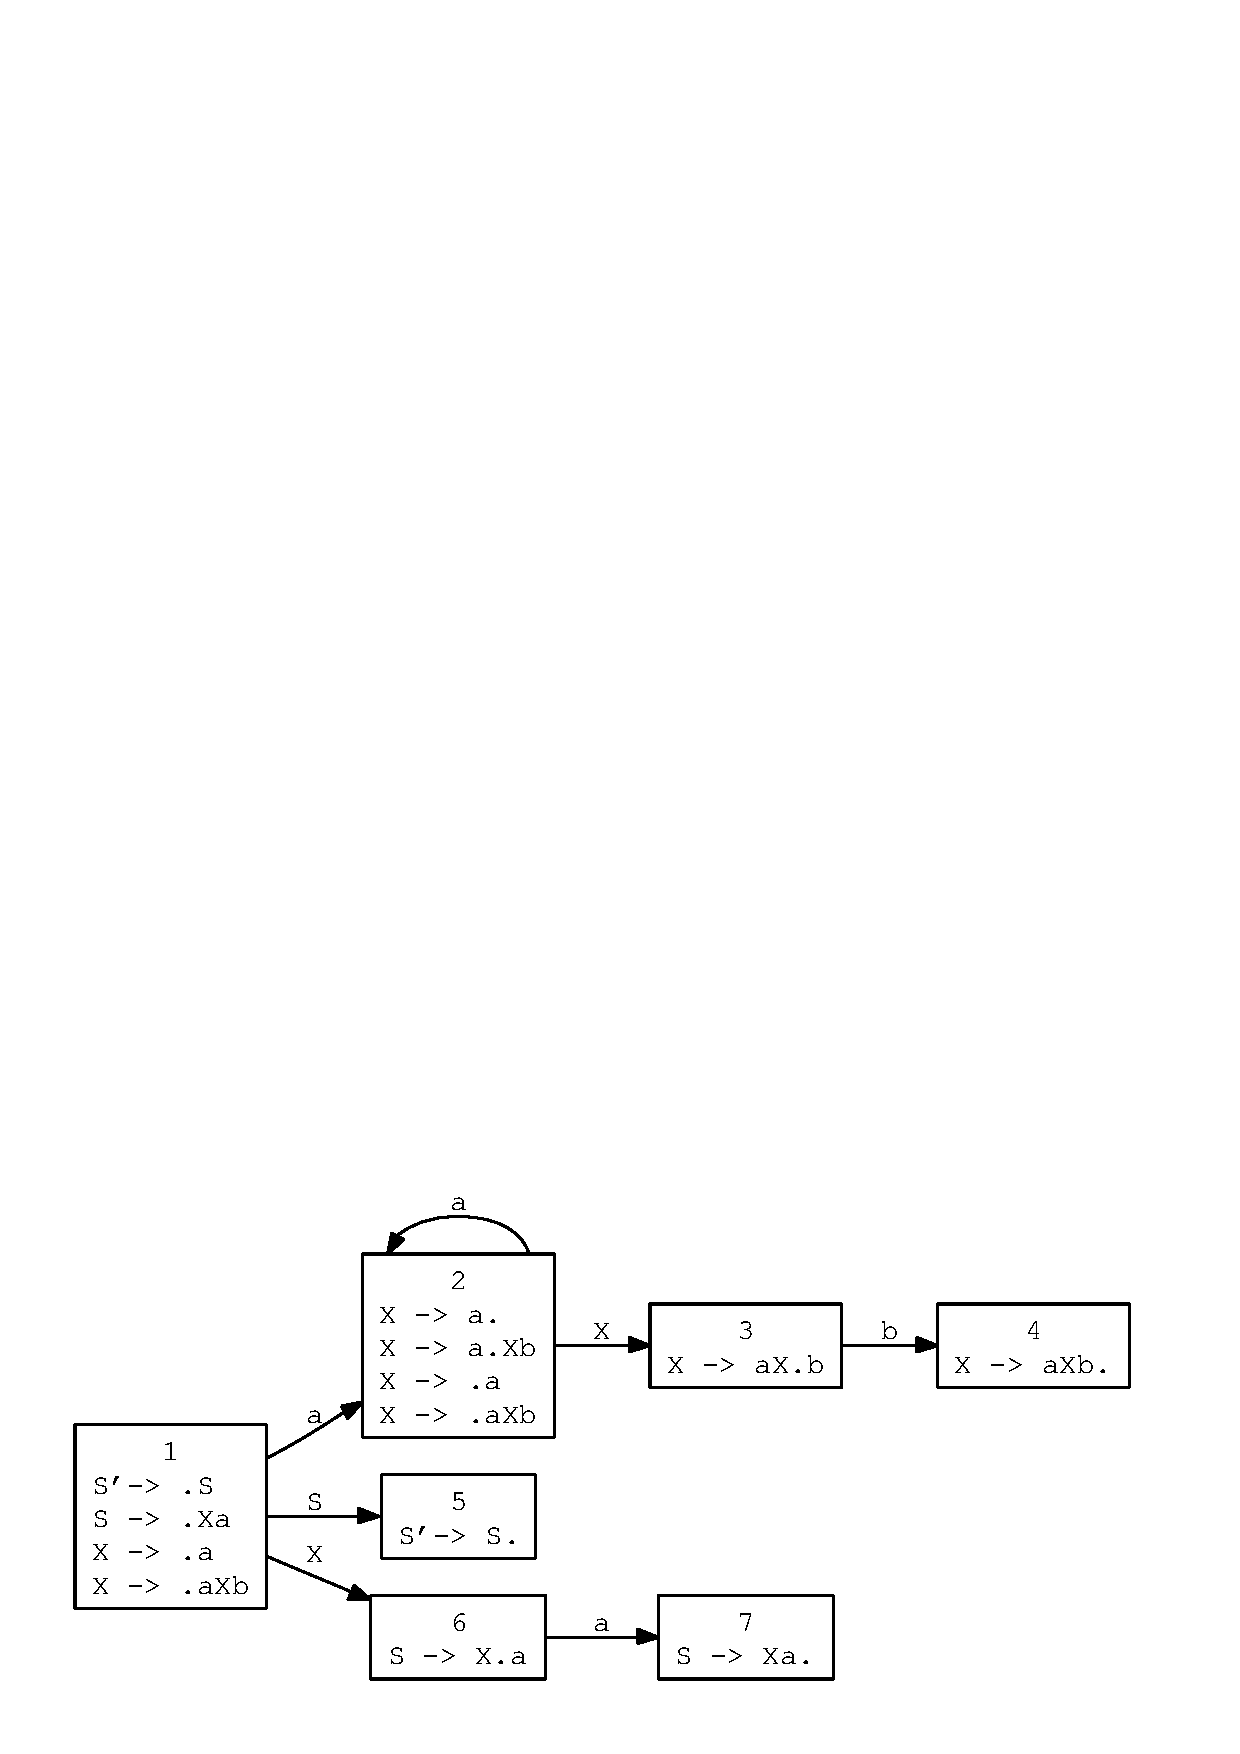
\includegraphics[scale=0.7]{viable-prefix-dfa.pdf}
\caption{A DFA for viable prefixes of the grammar in Question
\ref{slr}.}
\label{viable-prefix-dfa}
\end{center}
\end{figure}

\item Identify a shift-reduce conflict in this grammar under the
SLR(1) rules.

The First and Follow sets of the non-terminals in the grammar are as
follows.
\[
\begin{array}{ll}
\mathrm{First}(S) = \{ \mathbf{a} \}
& \mathrm{Follow}(S) = \{ \textbf{\$} \} \\
\mathrm{First}(X) = \{ \textbf{a} \}
& \mathrm{Follow}(X) = \{ \textbf{a}, \textbf{b} \}
\end{array}
\]

In the DFA state $2$, one valid action for an SLR(1) parser would be
to shift \textbf{a}.  Also, the parser could reduce using the
production $X \rightarrow \textbf{a}$ on the lookahead symbol
\textbf{a}, because \textbf{a} is in the Follow set of the
non-terminal $X$.

\item Assuming that an SLR(1) parser resolves shift-reduce conflicts
by choosing to shift, show the operation of such a parser on the input
string \textbf{aaba}.

\[
\begin{array}{lll}
\mathrm{Configuration} & \mbox{DFA Halt State} & \mathrm{Action} \\
\hline
\mid \textbf{a a b a \$} & 1 & \mathrm{Shift} \; \textbf{a} \\
\textbf{a} \mid \textbf{a b a \$}
& 2 \quad \mbox{shift-reduce conflict}
& \mathrm{Shift} \; \textbf{a} \\
\textbf{a a} \mid \textbf{b a \$} & 2
& \mathrm{Reduce} \; X \rightarrow \textbf{a} \\
\textbf{a }X \mid \textbf{b a \$} & 3
& \mathrm{Shift} \; \textbf{b} \\
\textbf{a } X \textbf{ b} \mid \textbf{a \$} & 4
& \mathrm{Reduce} \; X \rightarrow \textbf{a} X \textbf{b} \\
X \mid \textbf{a \$} & 6 & \mathrm{Shift} \; \textbf{a} \\
X \textbf{ a} \mid \textbf{\$} & 7
& \mathrm{Reduce} \; S \rightarrow X \textbf{a} \\
S \mid \textbf{\$} & 5 & \mathrm{Reduce} \; S' \rightarrow S \\
S' \mid \textbf{\$} & & \mathrm{Accept}
\end{array}
\]

\item Suppose that the production $X \rightarrow \varepsilon$ is added
to this grammar.  Identify a reduce-reduce conflict in the resulting
grammar under the SLR(1) rules.

The item $X \rightarrow \textbf{.}$ will appear in the DFA state 2.
Now, in state 2, there will be two possible reductions on the
lookahead symbol \textbf{a}: $X \rightarrow \textbf{a}$ and
$X \rightarrow \varepsilon$.

\end{enumerate}

\end{enumerate}

\end{document}
